%%%%%%%%%%%%%%%%%%%%%%%%%%%%%%%%%%%%%%%%%%%%%%%%%%%%%%%%%%%%%
% ECE 445 SENIOR DESIGN TEMPLATE
%%%%%%%%%%%%%%%%%%%%%%%%%%%%%%%%%%%%%%%%%%%%%%%%%%%%%%%%%%%%%
\documentclass[letterpaper,10pt]{article}

%%%%%%%%%%%%%%%%%%%%%%%%%%%%%%%%%%%%%%%%%%%%%%%%%%%%%%%%%%%%%
% The preamble starts here.
% You can add other packages that you want to use by using
% \usepackage command in the preamble.
% However, DO NOT change the settings that are already placed
% below unless you really know what you are doing.
%%%%%%%%%%%%%%%%%%%%%%%%%%%%%%%%%%%%%%%%%%%%%%%%%%%%%%%%%%%%%

% some commonly used packages
\usepackage{graphicx}
\usepackage{color,soul}
\usepackage{amsmath}
\usepackage{amsthm}
\usepackage{amsfonts}
\usepackage{setspace}
\usepackage{longtable}
\usepackage{url}
\usepackage{float}
\usepackage{caption}
\usepackage{booktabs}  % professional-looking tables
\usepackage{multicol} %used for getting multicolumn without page-break
\usepackage{multirow}	% multi-row tables
\usepackage{array}		% define column format of a table
\usepackage[colorlinks=true,linkcolor=black,citecolor=black]{hyperref}
\usepackage[top=1in, bottom=1in, left=1in, right=1in]{geometry}% set the page margins to 1 inch

% use the fancyhdr package to maintain the format of the page numbers,
% which is useful when the text color is changed
\usepackage{fancyhdr}
\fancyhf{}
\renewcommand{\headrulewidth}{1pt}
\renewcommand{\footrulewidth}{0pt}
\fancyfoot[C]{\textcolor{black}{\thepage}}
\fancyhead[L]{
\includegraphics[width=2cm]{University-of-Illinois-logo.jpg}}
\fancyhead[R]{\small{Infantry I.F.F. Design Review - Meyers \& Prince}}

% paralist provides extended list environments
\usepackage{paralist}
\setlength{\plitemsep}{0pt}

% define the color for section and subsection titles
\usepackage{xcolor}
\definecolor{titlecolor}{RGB}{31,73,125}
\definecolor{subtitlecolor}{RGB}{79,129,189}

% change the style of the section and subsection titles
\usepackage{titlesec}
\titleformat{\section}{\color{titlecolor}\Large\bf}{\color{titlecolor}\thesection}{0.8em}{}
\titleformat{\subsection}{\color{subtitlecolor}\large\bf}{\color{subtitlecolor}\thesubsection}{1em}{}
\titleformat{\subsubsection}{\color{subtitlecolor}\normalsize\bf}{\color{subtitlecolor}\thesubsubsection}{1.2em}{}
\titlespacing{\section}{0pt}{0em}{0em}
\titlespacing{\subsection}{6pt}{0em}{0em}
\titlespacing{\subsubsection}{12pt}{0em}{0em}



% change the style of the table of contents
\usepackage{titletoc}
\titlecontents{section}[1.5em]{}{\contentslabel{1.5em}}{\hspace*{-1.5em}}{\titlerule*[0.5pc]{.}\contentspage}
\titlecontents{subsection}[3em]{}{\contentslabel{2.1em}}{\hspace*{-2.1em}}{\titlerule*[0.5pc]{.}\contentspage}
\titlecontents{subsubsection}[5.1em]{}{\contentslabel{2.7em}}{\hspace*{-2.7em}}{\titlerule*[0.5pc]{.}\contentspage}

% command for centering texts in a fixed width table cell
\newcommand{\centpcol}{\leftskip\fill \rightskip\fill}

% command for setting the style of the appendix titles
\newcommand{\setappenstyle}{
	\titleformat{\section}{\color{titlecolor}\Large\bf}{\color{titlecolor}Appendix \Alph{section}}{0.8em}{}
	\titlecontents{section}[0em]{}{Appendix \thecontentslabel \hspace{1em}}{}{\titlerule*[0.5pc]{.}\contentspage}
}

% define the style of the title of the paper
\newcommand{\thetitle}[1]{\title{\begin{huge}{\bf #1}\end{huge} \color{subtitlecolor}\rule[25pt]{\textwidth}{1pt}}}

% define the style of the author
\newcommand{\theauthor}[3]{
	\author{\vspace{.4in}\\
	\textcolor{black}{By}\\
	#1
	\vspace{1in}\\
	\textcolor{black}{ECE 445 Design Review -} #2\\
	\textcolor{black}{TA:} #3
	\vspace{1in}}
}

% define the style of figure's caption
\newcommand{\figcap}[1]{
	\captionsetup{format=plain,font={small,color=subtitlecolor,singlespacing},margin={0pt,0pt}}
	\caption{\textcolor{subtitlecolor}{#1}}
	\vspace{-5pt}
}

% define the style of table's caption
\newcommand{\tablecap}[1]{
	\captionsetup{format=plain,font={bf,normalsize,singlespacing,color=black},margin={0pt,0pt}}
	\caption{\textcolor{black}{#1}}
	\vspace{-5pt}
}


\newcommand{\buildtoc}{
	\clearpage
	\singlespacing
	\tableofcontents
	\onehalfspacing
}

% set indentations and the space between paragraghs
\setlength{\parindent}{0pt}
\setlength{\parskip}{8pt}

\setcounter{secnumdepth}{4}

\titleformat{\paragraph}
{\normalfont\small\bfseries\color{subtitlecolor}}{\theparagraph}{1em}{}
\titlespacing*{\paragraph}
{18pt}{3.25ex plus 1ex minus .2ex}{1.5ex plus .2ex}

%%%%%%%%%%%%%%%%%%%%%%%%%%%%%%%%%%%%%%%%%%%%%%%%%%%%%%%%%%%%%
% PREAMBLE ENDS HERE, DOCUMENT STARTS BELOW
%%%%%%%%%%%%%%%%%%%%%%%%%%%%%%%%%%%%%%%%%%%%%%%%%%%%%%%%%%%%%

\begin{document}

% don't change these
\pagestyle{empty}
\doublespacing

% put the title of your project here. DO NOT include the brackets.
\thetitle{{I.F.F. (Identification Friend or Foe) System}}

% put your names here. seperate by \\. DO NOT include the brackets.
\theauthor{
	{Eric Meyers (emeyer7)}\\
	{Noah Prince (nprince2)}\\
}
{ % put the semester info here. DO NOT include the brackets.
	{Spring 2016}
}
{ % put your TA's name here. DO NOT include the brackets.
	{Braedon Salz}
}

% put the date and project number here. DO NOT include the brackets.
\date{
{February 29th, 2016}\\
Project No. 11
\clearpage
}

% don't change these
\maketitle
\pagestyle{fancy}
\begin{spacing}{1.15}


% build the table of contents. 
\color{black}
\buildtoc
\pagenumbering{gobble}
\clearpage
\setcounter{page}{1}
\pagenumbering{arabic}

%SECTION - Introduction
\section{Introduction}
\subsection{Statement of Purpose}
There have been several friendly fire incidents in recorded military history, accounting for an estimated 2\% to 20\% of all casualties in battle\textsuperscript{\cite{USArmy}}. Using attire to identify friend vs enemy is problematic in situations when both sides are clad in the same camouflage pattern, or are obscured by obstacles.

The purpose of this project is to create a system that quickly and accurately identifies friendly targets among military personnel on foot. Similar systems exist for aircraft, however not many exist for infantry.

The idea is to develop a two-way communication system so that when a soldier aims their weapon in the direction of a friendly target, they will receive notification through an LED that the target is, indeed, friendly and not an enemy. Throughout this document the infantry unit with the weapon will be referred to the "friendly interrogator" and the target will  be referred to as the "friendly target". 

This communication protocol can be 
\subsection{Objectives}
\subsubsection{Goals and Benefits}
\begin{itemize}
	\item Reduce number of friendly fire accidents during combat \textsuperscript{\cite{Garrison}}
	\item Reduce number of misfires accidents during combat \textsuperscript{\cite{Garrison}}
	\item Notify friendly personnel location of particular friendly target when aiming
	\item Other applications including but not limited to:
	\begin{itemize}
		\item Paintball or Airsoft
		\item Arcade Laser Tag
	\end{itemize}
\end{itemize}
\subsubsection{Functions and Features}
\begin{itemize}
	\item Laser diode on friendly interrogator to transmit unique I.D. of friendly interrogator.
	\item Photodiodes on friendly target to detect unique I.D. and verify it is a valid signal.
	\item R.F. Transmitter on friendly target to send acknowledgement back to interrogator.
	\item R.F. Receiver on friendly interrogator to verify that the target is friendly.
	\item LED on friendly interrogator to indicate to the operator the status of the target.
\end{itemize}
\clearpage

%SECTION - Design
\section{Design}
%Subsection - Block Diagrams
\subsection{Block Diagrams and Descriptions}
\subsubsection{System Overview}
The following figure represents the system as a whole, including both the friendly interrogator unit and the friendly target unit. Both units will be expanded upon in further detail below.
\begin{figure} [H]
	\centering
	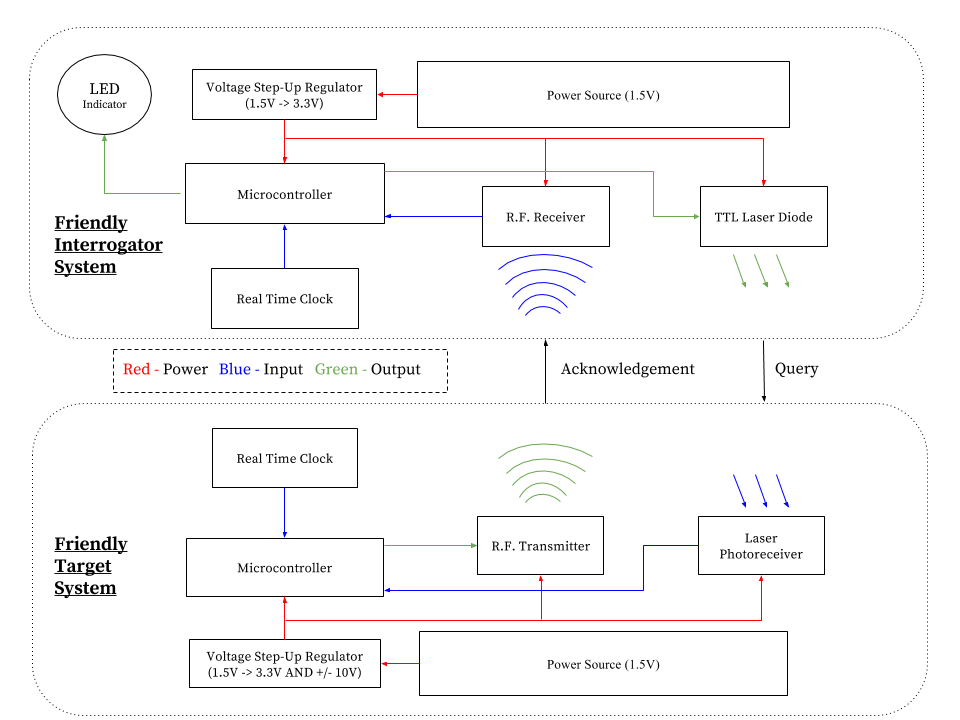
\includegraphics[scale=0.45]{System_Block_Diagram.png}
	\caption{System Block Diagram\label{fig:system-block-diagram}}
\end{figure}

%DESIGN - FRIENDLY INTERROGATOR UNIT
\subsubsection{Friendly Interrogator Unit}
The following diagram shows the friendly interrogator unit \textit{only}. The interconnections in red represent power, interconnections in blue represent input to a block and interconnections in green represent output to a block. These inputs and outputs are described below under each block description.
\begin{figure} [H]
\centering
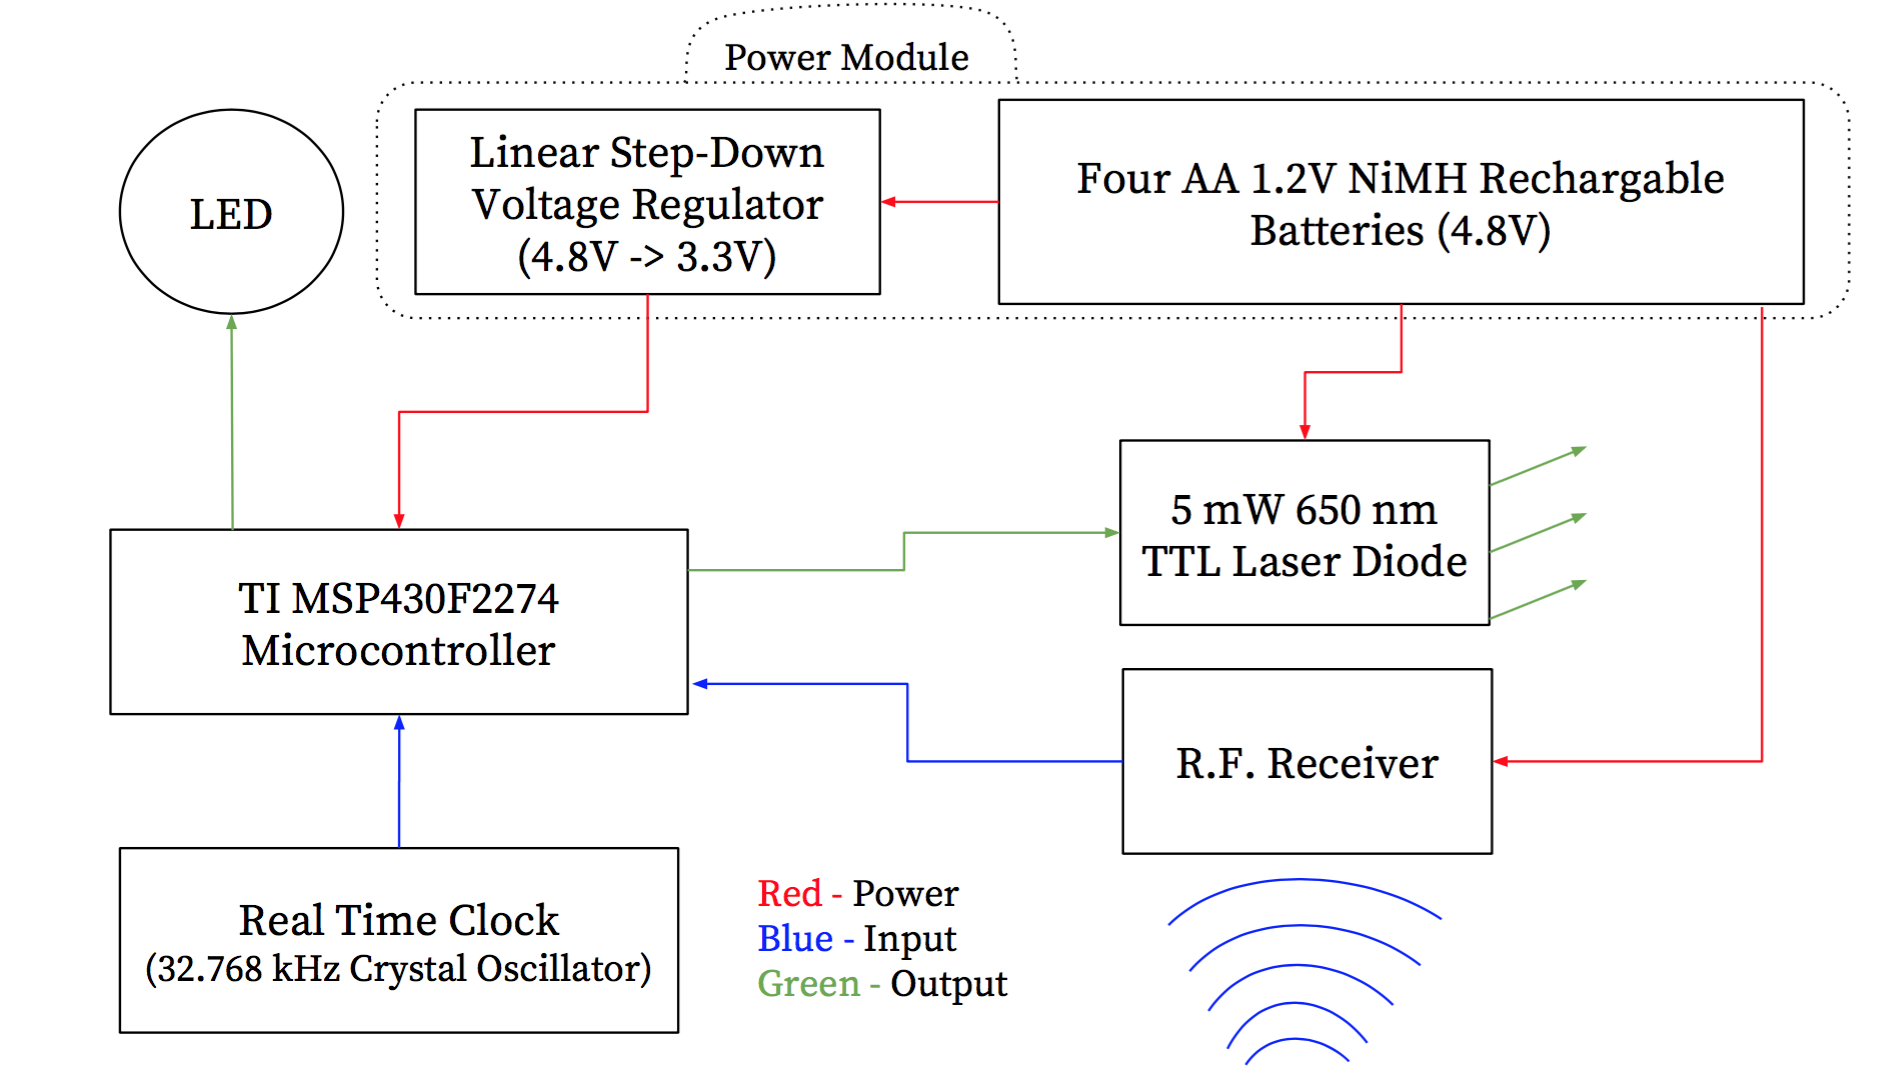
\includegraphics[scale=0.50]{Friendly_Interrogator_Block_Diagram.png}
\caption{Block Diagram of Friendly Interrogator Unit\label{fig:friendly-interrogator-block}}
\end{figure}

\normalsize\textbf{Power Module} \\ 
Power-In: N/A \\
Power-Out: Microcontroller Unit (3.3V), Laser Diode (4.8V), R.F. Receiver (4.8V) \\
Input(s): N/A \\
Output(s): N/A

The Power Module will consist of four standard rechargable 1.2V AA NiMH batteries which will provide a voltage of 4.8 when placed in series in a battery pack. This will then feed into a LD1117V33 Voltage Step-Down Regulator to bring the voltage to 3.3V. This 3.3V is necessary to provide the Microcontroller the correct voltage. The voltage regulator will provide a maximum of 900 mA of current which is well sufficient for this project. The schematic for the voltage regulator is depicted in Figure \ref{fig:ld1117-voltage-regulator-circuit}.

Depending on the manufacture chosen and the battery model, the batteries will hold a capacity of 1000 mAh to 3000mAh. For budgetary purposes the team will choose the ladder (a battery with a smaller capacity) because this will easily satisfy the requirements of powering the module for minimum of 8 hours. \hl{maybe show calculation???} The friendly interrogator unit will not be drawing much current however there are restraints placed on the current drawn from this battery in order to satisfy the time requirement. A 1000mAh battery will supply a circuit with 125 mA for 8 hours, therefore this unit must not draw more than 125 mA, which will be achievable.

The team decided to use four standard AA 1.2V NiMH rechargable batteries instead of any other standard batteries (such as disposable AAA or AA or a 9V battery) for several reasons. For one, the laser diode (as discussed later on) operates on a voltage from 4.5 - 5.5 voltage and this will satisfy this requirement. Also, the capacity is much higher for AA rechargeable batteries than 9V batteries so therefore the team went with the obvious option of choosing the AA batteries.

\hl{discuss case and mount???} \\
\hl{discuss switch and power-on process? 
	-the friendly target should on at all times once the operator turns it o
	-the friendly interrogator unit should only should turn on when the operator triggers it (i.e. the laser should not be constantly pulsing, it should only be when the interrogator wants to check the target status) - switch would solve this\\
	im not really sure how to word/organize all of this?}

\begin{figure} [H]
	\centering
	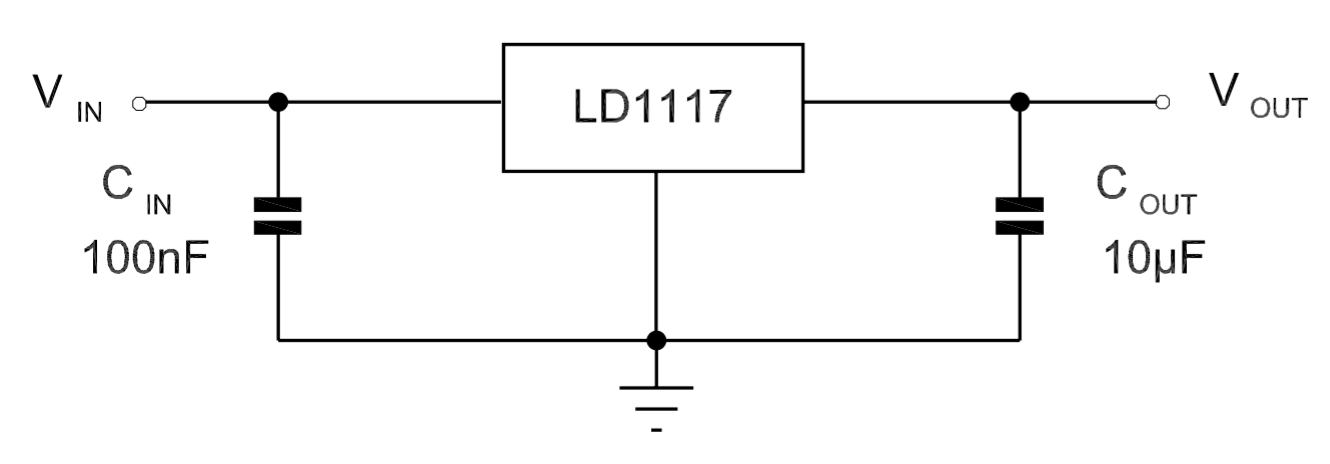
\includegraphics[scale=0.45]{LD1117_Voltage_Regulator_Circuit.png}
	\caption{System Block Diagram\label{fig:ld1117-voltage-regulator-circuit}}
\end{figure}

\normalsize\textbf{Microcontroller} \\
Power-In: 3.3V (from Power Module) \\
Power-Out: ?? \\
Input(s): Received R.F. Signal, Real Time Clock (32.768kHz Crystal Oscillator) \\
Output(s): LED, 5mW 650nm Laser Diode

The team chose to work with an T.I. MSP430F2274 Microcontroller Unit \textsuperscript{\cite{MSP430F2274}} due to its compiler simplicity, its availability in the ECE445 Senior Design Labs (inventory) and the number of GPIO Pins on board (compared to other options, this model had several I/O pins and was the most inexpensive). Compared to many other MCUs on the market, the MSP430 is relatively well documented and there exist several support forums on the internet to assist the team throughout the duration of the project.

The board requires a 3.3V power supply which is why the voltage regulator is necessary as stated before.

Please refer to Section \ref{section-functionality} to view in-depth discussion about the functionality of the MSP430F2274 Microcontroller Unit and how it will be used throughout this project.

\hl{INDICATE WHICH PINS ARE ACTIVE AND WHICH PINS ARE NOT BEING USED}
\hl{Indicate what the overall block layout of this is, i.e. show the Power Pins, the RX Pins, and the Laser Diode Pins}
\begin{figure} [H]
	\centering
	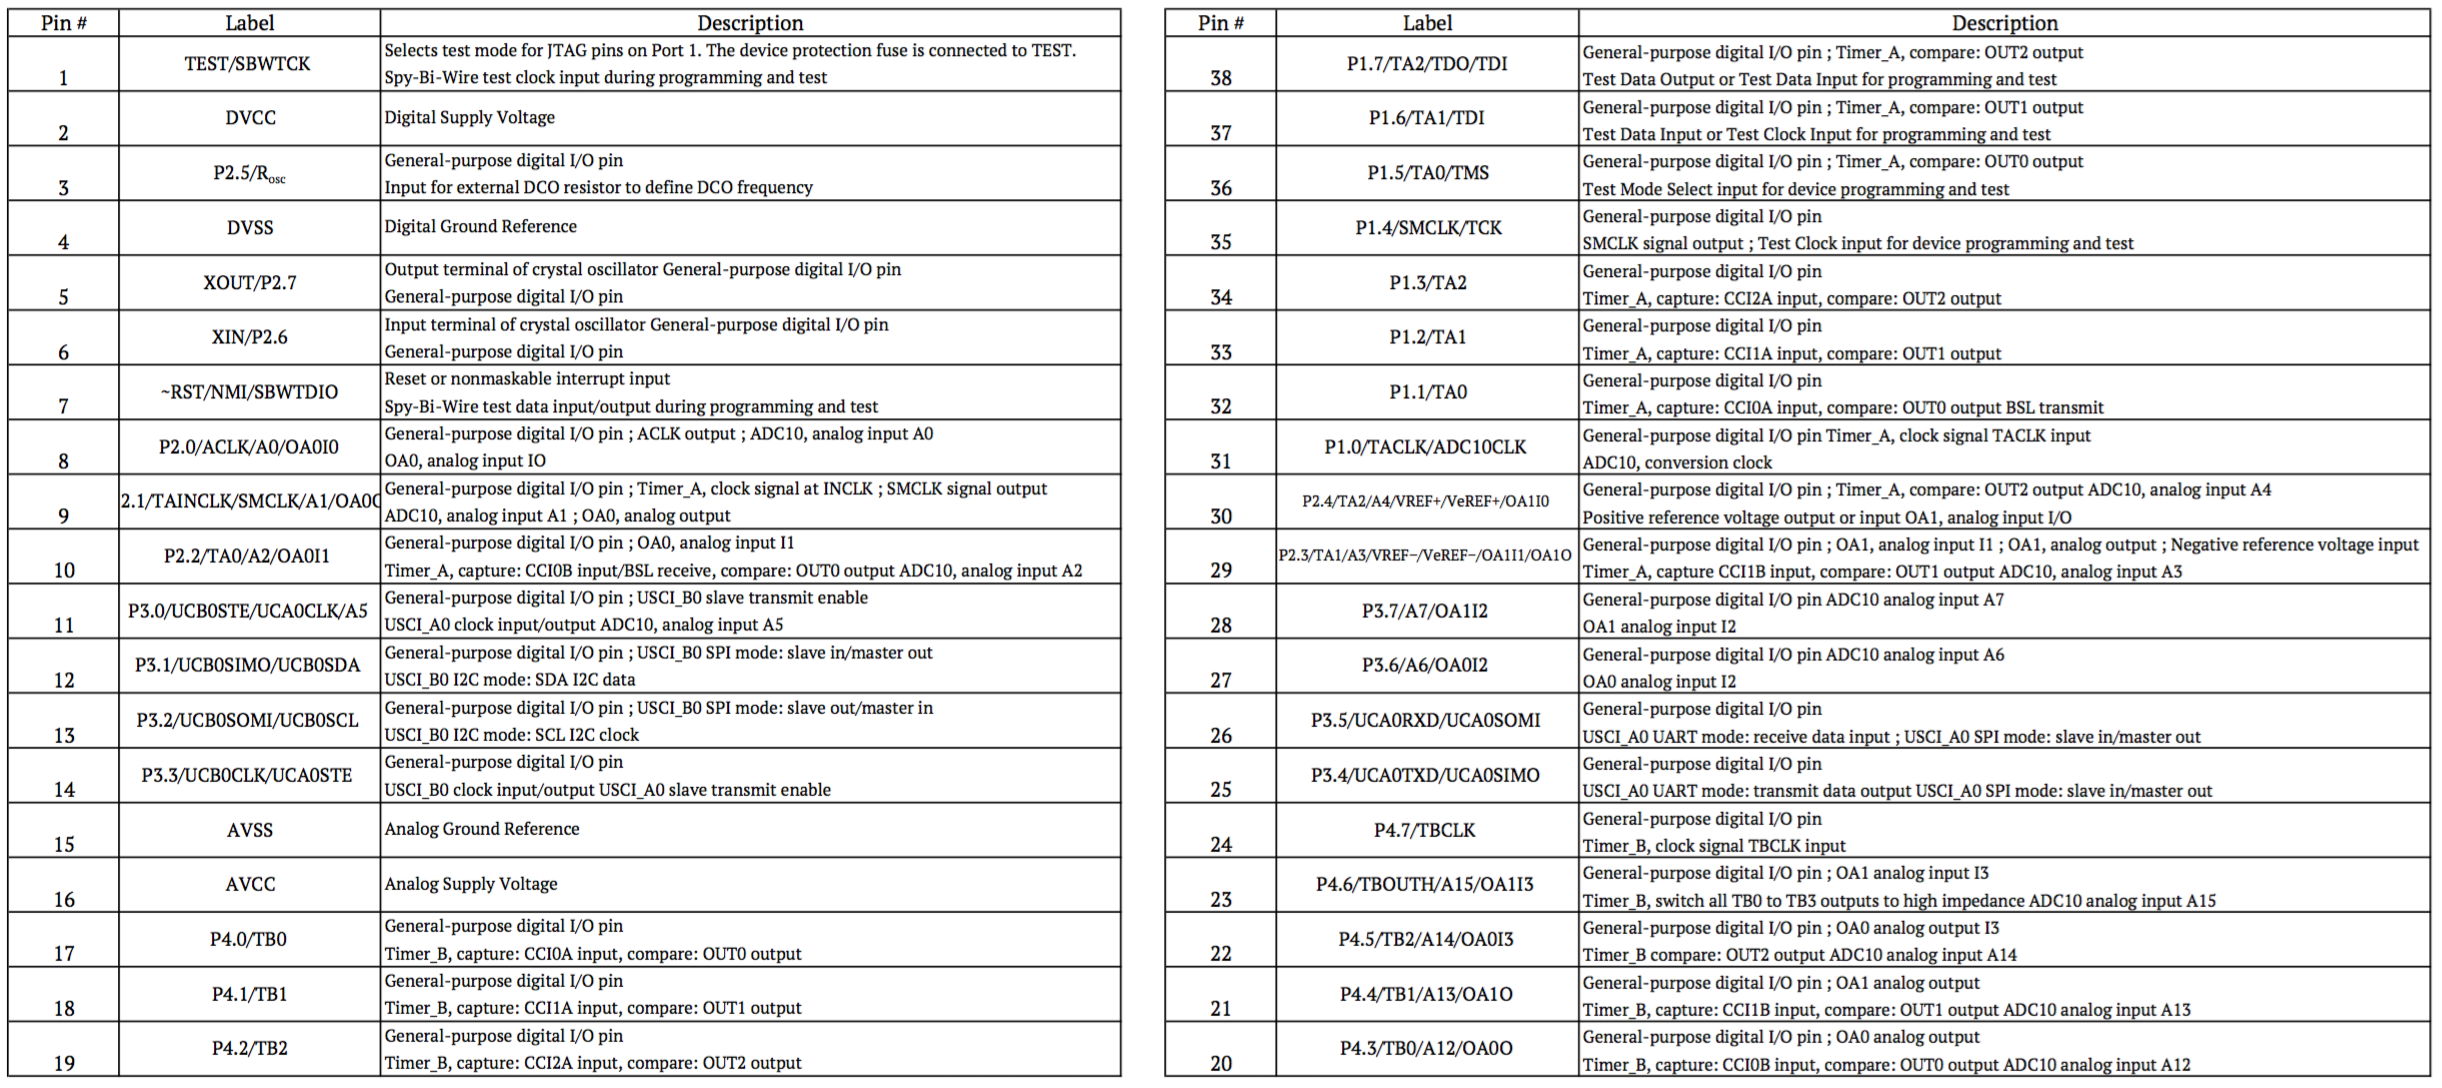
\includegraphics[scale=0.40]{MSP430_Pin_Layout.png}
	\caption{Pin Layout Table\label{fig:msp430-pin-layout}}
\end{figure}

\normalsize\textbf{Real Time Clock}\\
Power-In: N/A \\
Power-Out: N/A \\
Input(s): N/A \\
Output(s): Microcontroller

The Real Time Clock is not entirely necessary for the operation of the Laser Transmitter Subsystem, however it will be necessary for the operation of the R.F. Receiver and thus must be included in the MCU circuit. It will operate using a 32.768 kHz Crystal Oscillator (as recommended by T.I. \textsuperscript{\cite{RTC-Implementation}}) with an accuracy of +/- 20 PPM (deviates between 32.7673 kHz and 32.7687 kHz).

\normalsize\textbf{Laser Diode}\\
Power-In: \\
Power-Out: \\
Input(s): Microcontroller TTL Input /hl{change}\\
Output(s): 5mW Laser Beam 

The 5mW laser diode will operate on 3.3V at 25mA so a 1.3k$\Omega$ (confirm?) resistor is necessary to drop the current being supplied to the diode down to this threshold. 

Due to safety and ethical considerations, the requirements have changed for the divergence of the beam. The proposal stated a requirement of a 5-6 ft diameter beam at 50, 150, and 300 m (with optical adjustments allowed). This was assuming the team was using a 20mW laser diode which is now not the case (this design choice will  be discussed in both Section \ref{section-safety-ethics} and Section \ref{section-simulations-calculations} as appropriate). Instead the team will be using a 5 mW laser which will produce a beam divergence of 2.5-2.75 feet at \_\_\_\_ feet. 

Again, please refer to Section \ref{section-safety-ethics} and Section \ref{section-simulations-calculations} to view an in-depth discussion about these design choices.

\normalsize\textbf{R.F. Receiver} \\
Power-In: 4.8V (from Power Module) \\
Power-Out: N/A \\
Input(s): \\
Output(s):

A Linx 315 MHz LR Series R.F. Receiver will be used for this project along with a Linx 315-SP Splatch PCB Mounted Antenna.

\begin{table}[htbp]
	\centering
	\begin{tabular}{c|c}	% ccccccc indicates 7 center aligned columns
		\toprule	% top separator
		Parameter & Typical Value \\
		\midrule
		Receiver Frequency & 315 MHz \\ 
		Receiver Sensitivity & -112 dB \\
		R.F. Input Impedance & 50 $\Omega$ \\
		Receiver Turn-On Time & 7.0 ms  \\
		\bottomrule	% bottom separator
	\end{tabular}%
	\caption{Notable Datasheet Values for Linx 315 MHz LR R.F. Receiver}
	\label{tab:table2}	% this is the label given to the table that can be referenced using \ref{tab:Exp1Part1_7}
\end{table}%


%DESIGN - FRIENDLY TARGET UNIT
\subsubsection{Friendly Target Unit}

\begin{figure} [H]
	\centering
	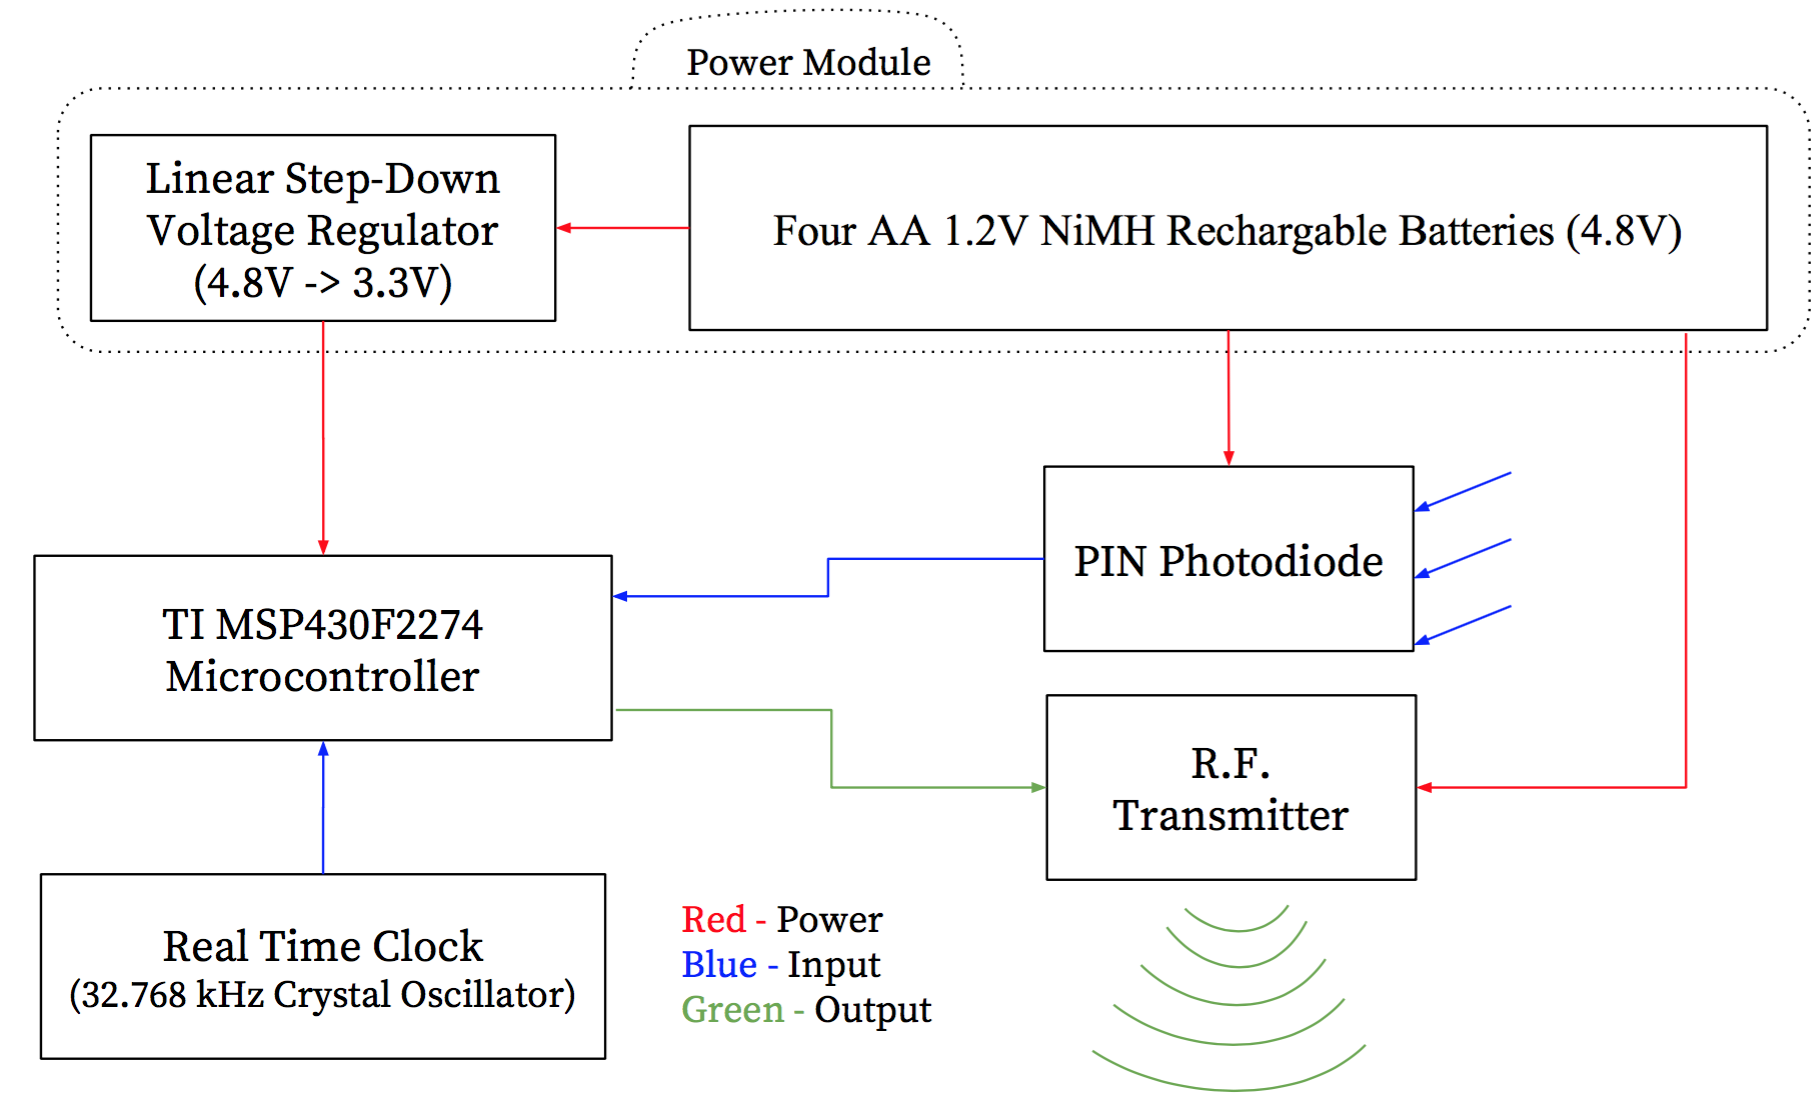
\includegraphics[scale=0.50]{Friendly_Target_Block_Diagram.png}
	\caption{Block Diagram of Friendly Target System\label{fig:friendly-target-block}}
\end{figure}

\normalsize\textbf{Power Module} \\
Power-In: N/A\\
Power-Out: \\
Input(s): \\
Output(s):

The power module on board the Friendly Target Unit will be the same as the Friendly Interrogator Unit. Th Please reference that section to get all details pertaining to the power module.


\normalsize\textbf{Microcontroller} \\
Power-In: \\
Power-Out:\\
Input(s):\\
Output(s):\\
\hl{INDICATE WHICH PINS ARE ACTIVE AND NOT}

\normalsize\textbf{Real Time Clock} \\
Power-In: \\
Power-Out: \\
Input(s): \\
Output(s):

The Real Time Clock on board the Friendly Target Unit will be the same as the Friendly Interrogator Unit. Please reference that section to get all details pertaining to the Real Time Clock.

\normalsize\textbf{Laser Photodiode}\\
Power-In: \\
Power-Out: \\
Input(s): \\
Output(s):

\normalsize\textbf{R.F. Transmitter}\\
Power-In: \\
Power-Out: \\ 
Input(s): \\ 
Output(s):

A Linx 315 MHz LR Series R.F. Transmitter will be used for this project along with a Linx 315-SP Splatch PCB Mounted Antenna. This is an identical setup to the receiver end on the friendly interrogator unit as discussed before. 

The 

\begin{table}[htbp]
	\centering
	\begin{tabular}{c|c}	% ccccccc indicates 7 center aligned columns
		\toprule	% top separator
		Parameter & Typical Value \\
		\midrule
		Transmit Frequency & 315 MHz \\ 
		Output Power & 4 dB \\
		Data Rate & 10,000 bps \\
		R.F. Output Impedance & 50 $\Omega$ \\
		Transmitter Turn-On Time & 1.0 ms  \\
		\bottomrule	% bottom separator
	\end{tabular}%
	\caption{Notable Datasheet Values for Linx 315 MHz LR R.F. Transmitter}
	\label{tab:table2}	% this is the label given to the table that can be referenced using \ref{tab:Exp1Part1_7}
\end{table}



%Subsection - Circuit Schematics
\subsection{Circuit Schematics}

\subsubsection{Friendly Interrogator Unit}
The circuit schematic is shown below for the Friendly Interrogator Subsystem.
\begin{figure} [H]
	\centering
	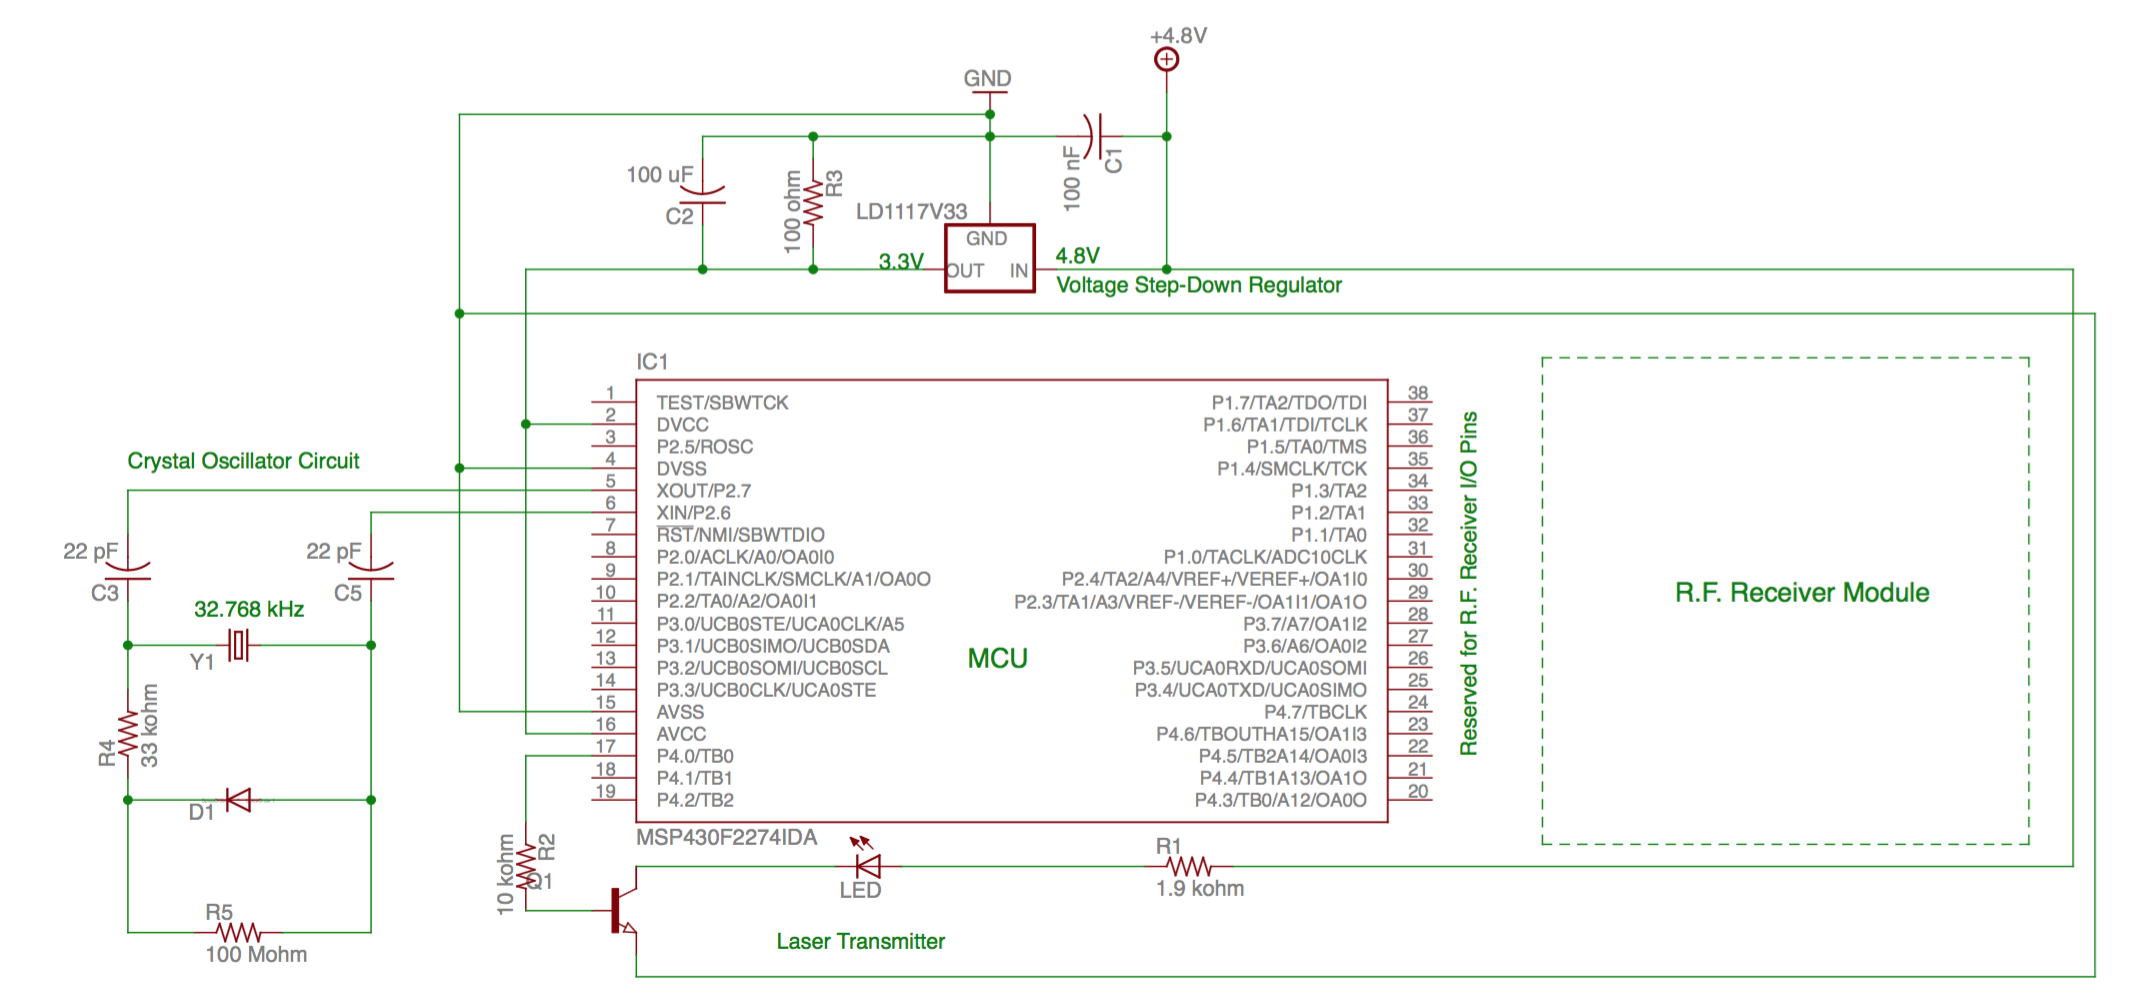
\includegraphics[scale=0.45]{Circuit_Schematic.png}
	\caption{Circuit Schematic of Laser Transmitter\label{fig:circuit-schematic}}
\end{figure}

\subsubsection{Friendly Target Unit}

\subsection{Functionality} \label{section-functionality}
\hl{Do we need any setup procedures?}
This section is to explain the overview of how each part interfaces with another and the protocol used to transmit data from both the friendly interrogator unit to the friendly target unit. The below diagram is a flowchart representing the flow of events that occur to identify a target as friendly. Each individual label will be explained in extensive detail below.

\begin{figure} [H]
	\centering
	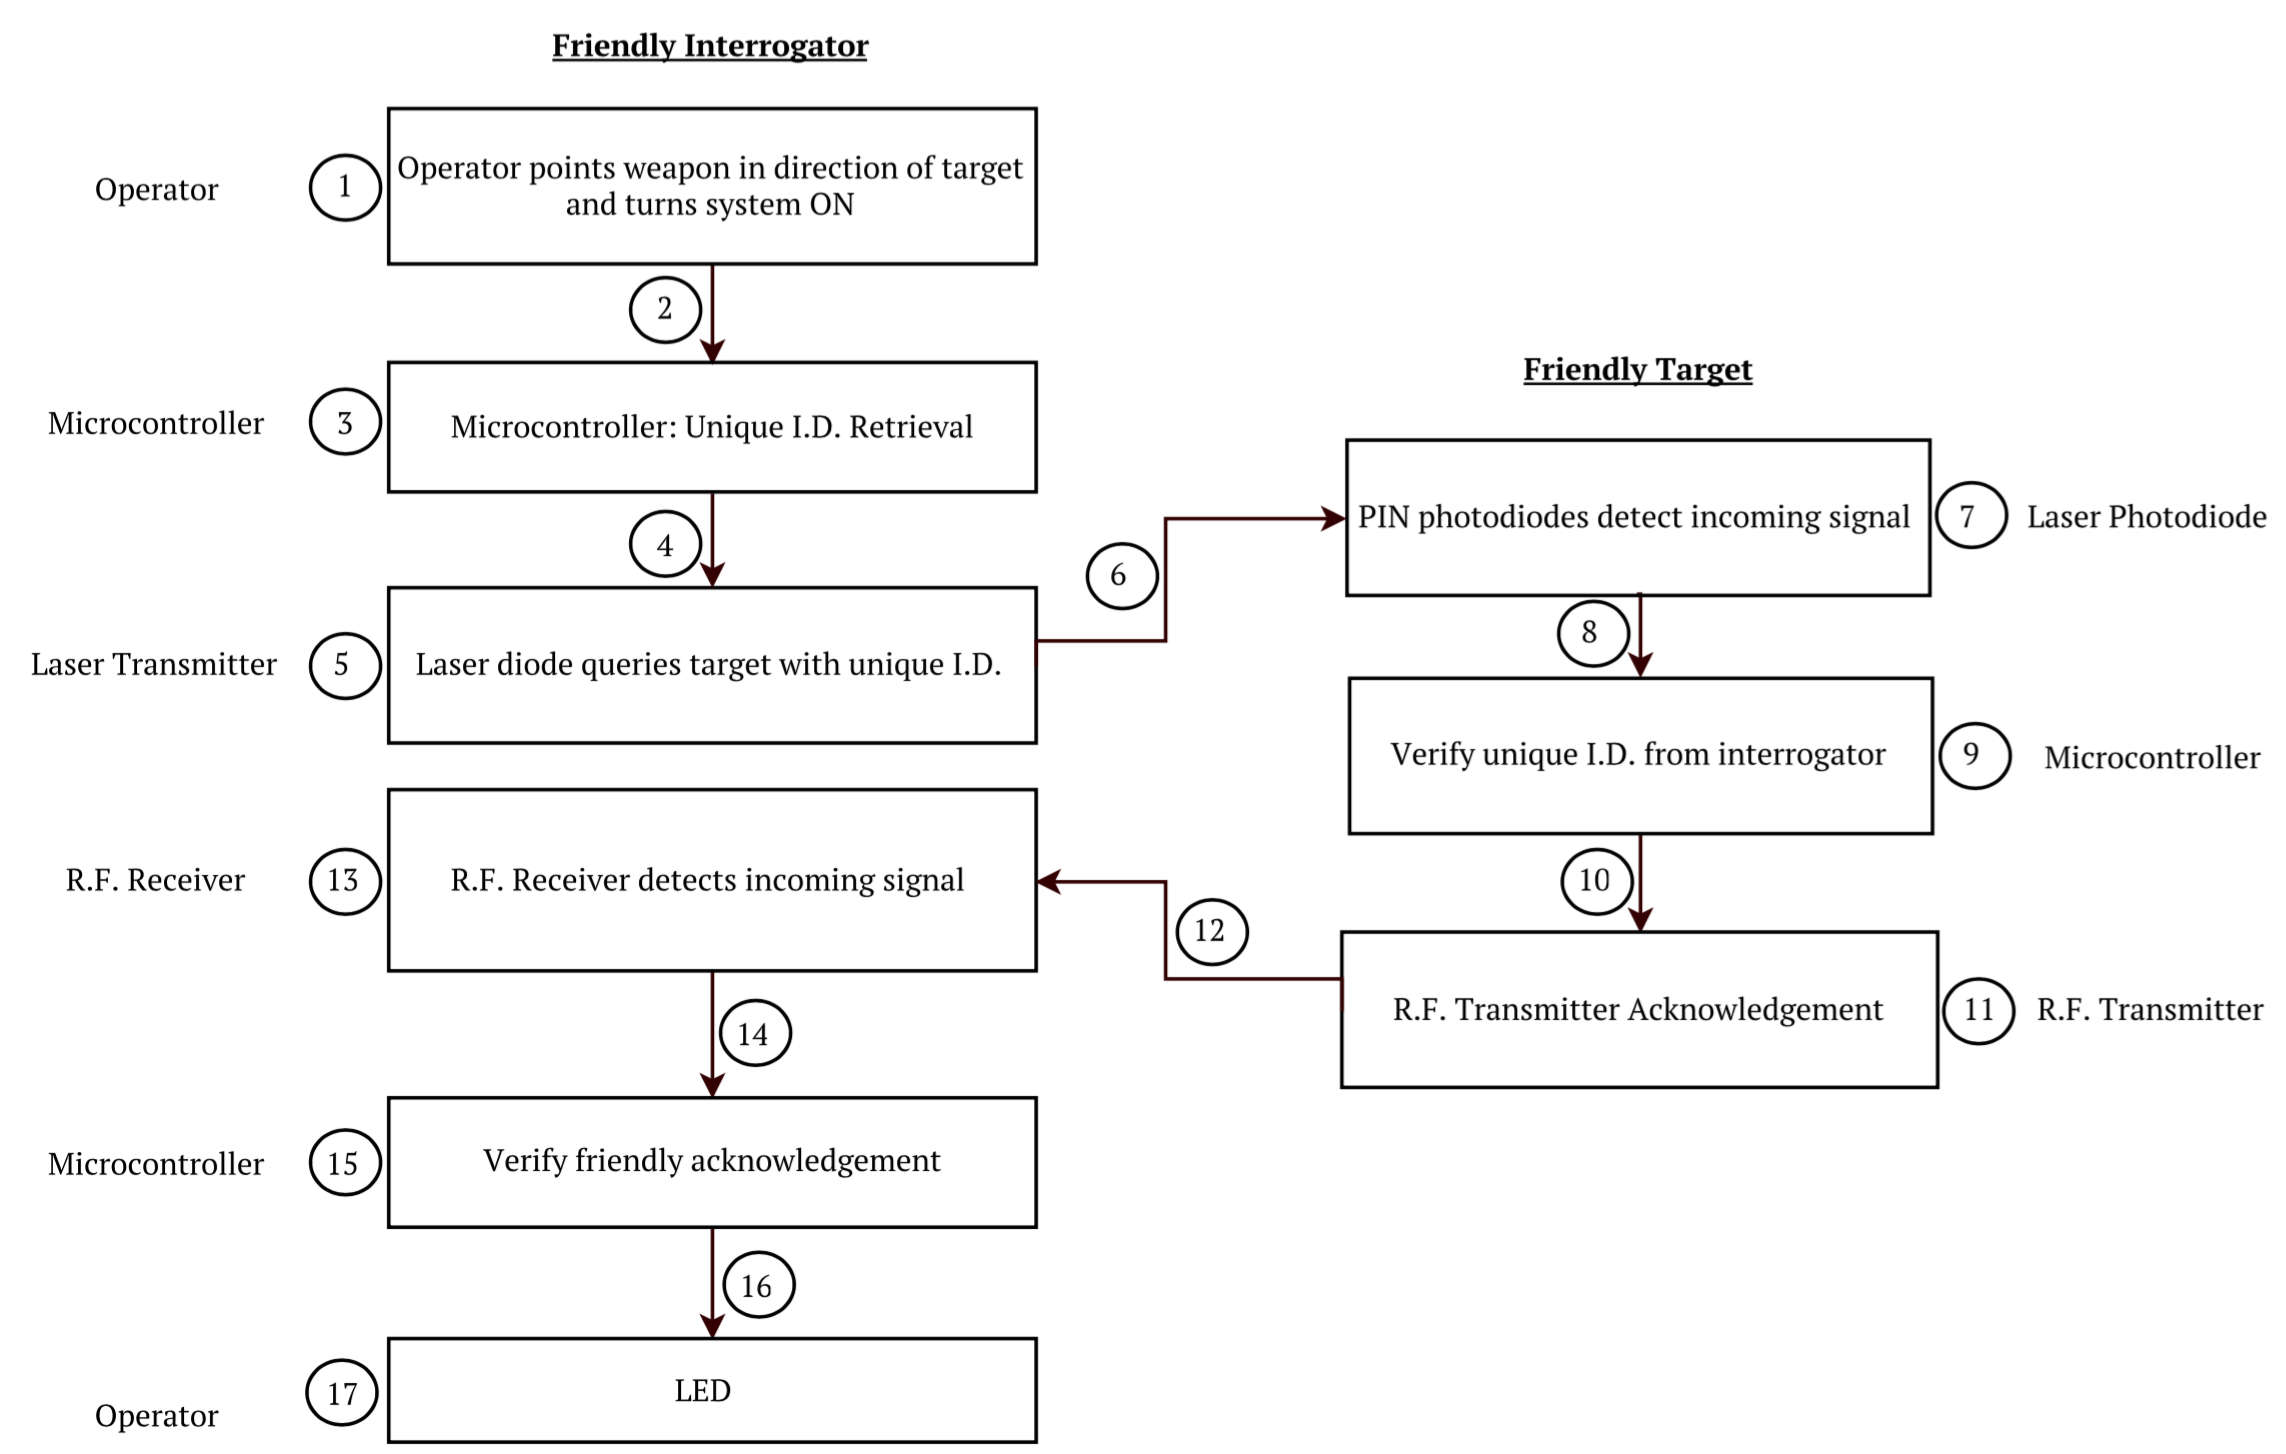
\includegraphics[scale=0.4]{Functional_Flowchart.png}
	\caption{Flowchart for Functionality\label{fig:circuit-schematic}}
\end{figure}

The left side of this diagram are all events that occur within the friendly interrogator unit, and the right side represents all of the events that occur on the friendly target side. This flow diagram also assumes that both the interrogator operator and the friendly target operator have powered on their respective units.

\normalsize\textbf{Event \#1 - Operator points weapon in direction of target and turns power ON}\\
The operator will trigger the power of the friendly interrogator unit which will then send a signal to the 

\subsection{Software Flowcharts}


\subsection{Numerical Analysis and Simulations/Plots} \label{section-simulations-calculations}

\subsubsection{Calculations}

\normalsize\textbf{Laser Diode} \\
With some tolerance, the PIN photodiode used in the friendly target system can register an irradiance of 9 $\frac{W}{m^2}$. The laser required to achieve this irradiance is a function of the laser power and the radius of the beam. With relatively short distances of 0-300 m, atmospheric deflection of light is negligible. 

Using trigonometry, the power as a function of radius is given by $P = \pi r^2  E_{req} $, where $r$ is the radius (in meters) and $E_{req}$ is the required irradiance of 9 $\frac{W}{m^2}$. 

For a diameter equal to the one stated in the proposal ($\approx 1.6764 m$), a $\pi (0.8382)^2(9) \approx 20 mW$ laser is needed. A $20 mW$ laser is a Class 3B laser, and is considered dangerous. For the scope of this senior design project, a $5mW$ laser will be used instead. 

The radius achieved using a $5 mW$ laser is given by $\sqrt{\frac{P}{E_{req} \pi}} = 0.420522 m$. This is approximately a $2.75 ft$ diameter beam, which is still the size of a person's chest.

\subsubsection{Simulations/Plots}
\hl{INSERT PLOTS/ANY SORT OF ANALYSIS HERE}


%SECTION - Requirements and Verification
\section{Requirements and Verification}
\begin{figure} [H]
	\centering
	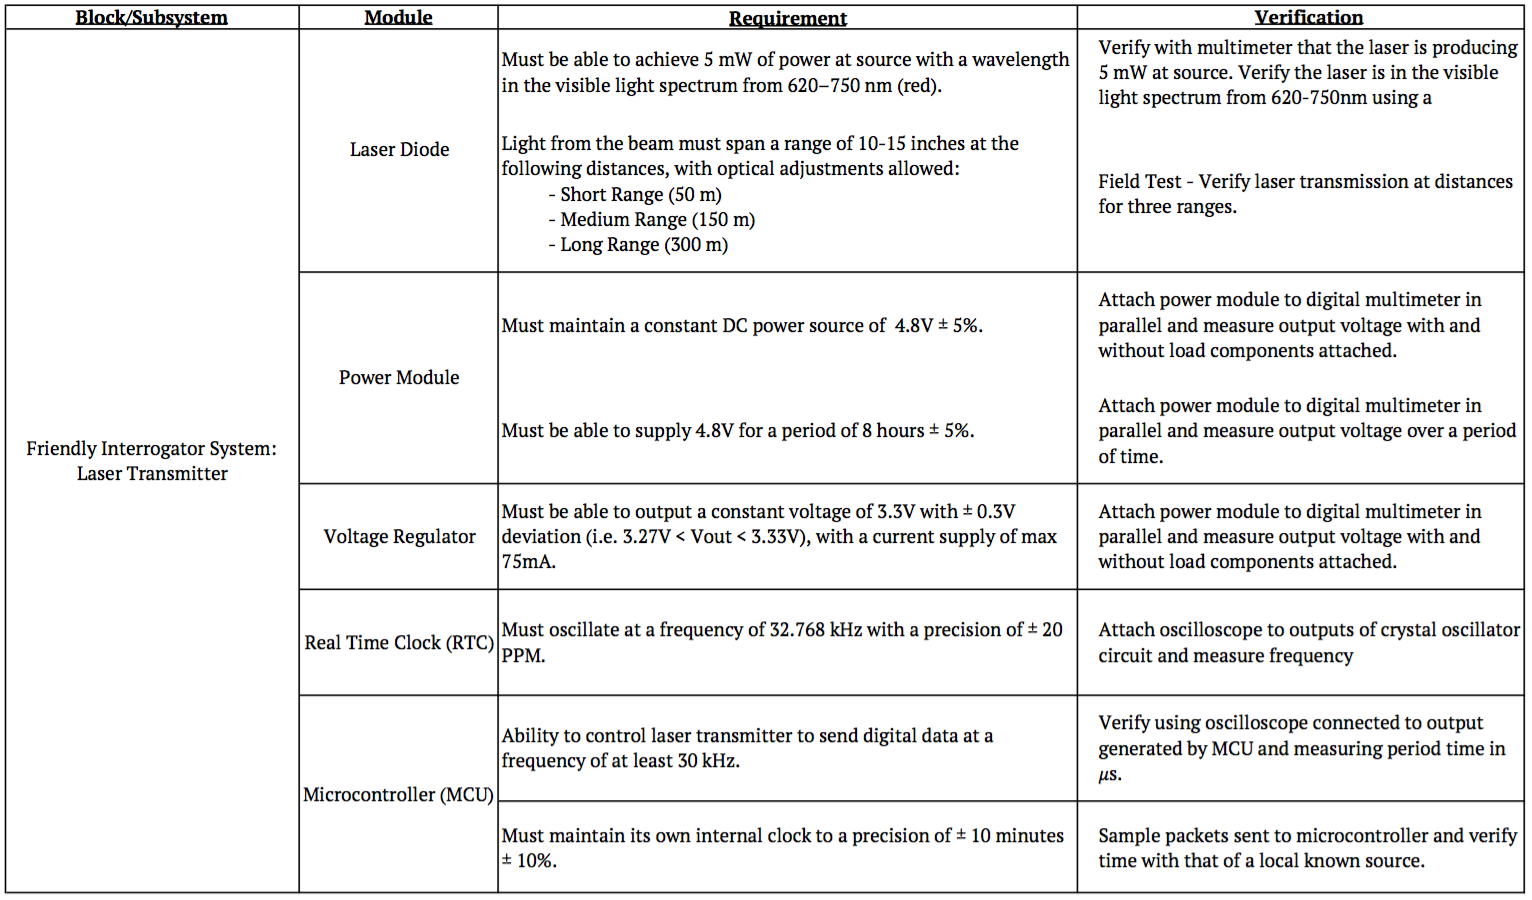
\includegraphics[scale=0.3]{Requirements.png}
	\caption{Requirements/Verification for Laser Transmitter System\label{fig:requirements}}
\end{figure}
\subsection{Tolerance Analysis}
\hl{NEED TO INCLUDE IN DEPTH ANALYSIS-\\
	Tolerance analysis is part of the DESIGN process. The tolerance analysis is not an experiment to see what the limits of your project are after it has been designed and built. The tolerance analysis is an exercise in working backwards from what your goal is, and then figuring out how precise a specific hardware component must be. "We will stress the device until it no longer works as intended and look at the results" is not a tolerance analysis. "Given that we have a goal of X, The accuracy of component Y must be Z to achieve X properly" is a tolerance analysis. It should involve math and design equations. For example, in amplifier design there is usually a bias circuit that includes a resistor network. Resistor values in real life are not exact and have an advertised tolerance (10\%, 5\%, 1\%). Find how accurate your resistors must be to meet your gain or bandwidth requirements in the worst case scenario. If it is lower than 10\%, you have just concluded that your design will require parts with a tighter tolerance.}

\subsection{Safety} \label{section-safety-ethics}
\normalsize\textbf{Laser Diode} \\
As stated previously, the proposal requirements would have required a $20mW$ IR laser. However, in the State of Illinois, a 20mW laser is considered a Class 3B laser and must be registered with the Division of Nuclear Safety in the Illinois Emergency Management Agency. This would have required the team to file the correct paperwork and pay a registration fee of \$50. This paperwork would have likely caused delays in receiving parts and construction of this project. A 20 mW laser would have also needed much more pre-caution and safety mitigations than a much less powerful laser.

For the reasons stated above, the team will instead use a $5mW$ visible red laser. $5mW$ visible lasers have a low chance of injuring the eye, as the blinking reflex will save a victim from permanent damage; as opposed to IR lasers which can go unnoticed for several seconds. 

The following is a calculation for the nominal ocular hazard distance (NOHD) of our laser, as defined by the ANSI Standard \cite{ANSI}.

The maximum permissible exposure (MPE), as defined by the ANSI Standard \cite{ANSI} is the highest power or energy density of a light source that is considered safe, i.e. that has a negligible probability for creating damage. This MPE for a pulsing laser is calculated as the minimum of the following three rules:

\begin{enumerate}
	\item Any single pulse in the train must not exceed the MPE for the pulse exposure time.
	\item The exposure from any group of pulses delivered in time T must not exceed the MPE for
	time T, where T is 0.25 seconds (from the blinking reflex), for a visible laser. 
	\item For thermal injury, the exposure for any single pulse within a group of pulses must not
	exceed the single-pulse MPE multiplied by a multiple-pulse correction factor
\end{enumerate}

The laser will pulse at a rate of 40 kHz. Assuming at most a 50\% duty cycle, each pulse will be of max length $1.25*10^{-5} s$. The divergence of the beam is smallest for the longest range; a lower divergence is more restrictive in terms of safety, so this calculation uses $300m$. The divergence of the beam for 300m is 2.79 mrad and the beam waist is approximately $4 mm$. \\

Following the ANSI Standard \cite{ANSI}, the Rule 1 calculation is 

{\large $5*10^{-3}*(\frac{2.79}{1.5})  = 0.0093 \frac{J}{m^2}$ }\\

The Rule 2 calculation is

{\large $\frac{18(.25^{0.75})(\frac{2.79}{1.5})}{.25*40000} = 0.0011837 \frac{J}{m^2}$ }\\

The Rule 3 calculation is

{\large $(.25*40000)^{0.25} * 5*10^{-3}*(\frac{2.79}{1.5}) = 0.093 \frac{J}{m^2}$ }\\

The most restrictive of all the rules is Rule 2, which gives us an MPE of $0.0011837 \frac{J}{m^2}$.

At $5mW$ with a pulse width of $1.25*10^{-5}$, the power of the laser is $6.25*10^{-8} J$. 

The NOHD is defined as

{\LARGE $ \frac{\sqrt{\frac{4 * P}{\pi * MPE}} - 2w}{\theta}$}

Where P is the power of the beam ($6.25*10^{-8} J$) and $w$ is the waist of the beam ($1mm$). This gives an NOHD of 

{\Large$ \frac{\sqrt{\frac{4 * 6.25*10^{-8}}{\pi * 0.0011837}} - 2(0.004)}{0.00279} = 0.0713 m $}

The team will avoid eye damage by not working with their eyes inside of 8 cm from the laser. If it is necessary to get this close to the laser, the team will wear eye protection or simply power off the laser. 


\subsection{Ethical Issues}


%SECTION - Cost and Schedule
\clearpage
\section{Cost and Schedule}

\subsection{Cost Analysis}
The labor cost was calculated as follows:

\begin{center}
	Labor Cost = Worker Salary (\$/hour) x 2.5 x Time (Hours) Invested In Project
\end{center}

\hl{COMPILE PARTS LIST, SUM UP TOTAL, ADD TO LABOR COSTS - SAME AS PROPOSAL}

\subsection{Schedule}
\hl{EDIT SCHEDULE CREATED IN PROPOSAL}


%SECTION - References
\clearpage
\bibliographystyle{IEEE_ECE}
% include the BibTex file here to build reference
\bibliography{Citations}\addcontentsline{toc}{section}{Reference}

\clearpage
\end{spacing}
\end{document}

